\documentclass[twoside,11pt,nolof]{starlink}

\stardoccategory  {Starlink User Note}
\stardocinitials  {SUN}
\stardocsource    {sun270}
\stardocnumber    {270}
\stardocauthors   {Sarah F. Graves}
\stardoccopyright {Copyright \copyright\ 2015 Science and Technology Facilities Council}
\stardocdate      {9th February 2015}
\stardoctitle     {Starlink Latex Suppport for pdf and html}
\stardocversion   {1.0}
\stardocmanual    {User's Guide}

\stardocabstract{ Documentation and advice for using the starlink.cls
  \LaTeX\ class and its TeX4HT configurations when building pdf and
  html starlink documentation.  }

% --------------------------------------------------------------------------
\begin{document}
\scfrontmatter

\section{Introduction}
\label{sec:intro}
\xlabel{intro}

% Write normal latex, with a few limitations
Starlink documents -- specifically Starlink User Notes (SUNs),
Starlink Guides (SGs), Starlink General Papers (SGPs) and Starlink
System Notes (SSNs) -- should be written using the
\texttt{starlink.cls} latex class. This is designed to allow output
into either PDF format (using pdflatex) or html format (using
htlatex/TeX4HT).


It should be pretty straightforward to write documents using this, as
most standard latex macros should work as usual. This class should
provide a fairly consistent look amongst all the documents, and both
output types.

By standardising on a single class, writers of starlink documents
should be able to concentrate on the content, without having to spend
much time tweaking the output. In addition, the more standardised the
documents are, the easier it will be to change either the appearance
(by tweaking only the class file), or to port documents to a different
system if that is ever required.

\subsection{Good practice}

\begin{description}
\item[Check both html output and pdf as you go] Please don't only
  check that your latex source builds correctly in pdf format. The
  html output is likely to be more widely used, and is a little more
  finicky about what it will work against than the pdf output is. You
  should, therefore, ensure your document both builds correctly as
  html, and also ensure that the formatting has succeeded in
  html. \textbf{Consider the html output as the most important version
    of the document.}

\item[Have an up-to-date version of the document] Before starting,
  make sure you've checked out the current version of the document. If
  you don't know how to use git, there are many tutorials online. If
  they don't suffice, you could ask any local git users, or local
  starlink developers, or do feel free to ask for advice on the
  starlink developers list about anything specific to starlink.

  Do make sure you're not editing a version of a .tex file you find
  from a release or rsynced build of starlink, as there could be later
  changes that have been made by other editors on the master GitHub
  Starlink repo.

\item[Commit regularly] Please don't spend months carefully crafting a
  perfect document, without regularly pushing any commits to GitHub or
  checking for updates. Other starlink contributors aren't psychic,
  and they may make their own substantial changes to the document in
  the mean time. This will leave you with a dificult merge to fix
  before you can push your own change.

\item[Use LaTeX commands] While many users use plain TeX commands when
  writing \LaTeX, these tend to be a little less well supported by
  TeX4HT, so can cause problems in the html output. Specific examples are:
  \begin{itemize}
  \item Use \verb+\texttt+ instead of \verb+\tt+
  \item Use \verb+\textrm+ instead of \verb+\rm+
  \item Use \verb+\emph+ instead of \verb+\em+
  \end{itemize}
\end{description}


If you are writing your document within a built Starlink tree, you can
use the usual 'make' command within the correct directory to build
the document. Usually these will print to screen the actual commands
that run, so you can run those manually if you want to.

If the above sentence makes no sense what-so-ever, and you've never
tried to build Starlink at all, never fear! The following
'Getting started' guide should help.

\subsection{Getting started if you're not a Starlink Programmer}

Some documents (especially instrument-specific cookbooks and documents
providing advice for general astronomer users) could do with help from
non-Starlink programmers. For example, JCMT support scientists are
often asked to help write cookbooks for JCMT instruments (see SC/21
and SC/20). Many SUNs consist of both a reference section and a users
guide, and contributions from any users who have suggested updates or
improvements to the users sections would be very welcome.


The following workflow is suggested:
\begin{description}
\item[clone the software repository from GitHub]
  (You'll only do this once, and afterwards go straight to the next step)

\item[Ensure the current check out is up-to-date with the GitHub repo]
  \texttt{git pull --rebase}

\item[Edit a file]

\item[Check it builds] If you ensure you have a (recent) starlink
  build available on your machine, then you can run the following
  commands to produce PDF and HTML output by setting the
  \texttt{STARLINK\_DIR} environment variable to point to your (e.g.)
  \file{star/} or \file{stardev/} directory.

  (Replace \texttt{sunXXX.tex} with the name of your \LaTeX file).
  \begin{aligndesc}
  \item[PDF]
\begin{terminalv}
TEXINPUTS=$STARLINK_DIR/share/latexsupport//: pdflatex sunXXX.tex
\end{terminalv}
\item[]
   \item[HTML]
\begin{terminalv}
TEXINPUTS=$STARLINK_DIR/share/latexsupport//: \
TEX4HTENV=$STARLINK_DIR/share/latexsupport/tex4ht.env \
TEX4HTHTF=:$STARLINK_DIR/share/latexsupport: htlatex sunXXX.tex \
"starlinkxhtml.cfg,charset="utf-8",fn-in" ' -cvalidate -cstarfont' ""
\end{terminalv}


   \end{aligndesc}

   You will have to have reasonably recent TeX distribution on your
   machine, with the majority of standard packages installed.

 \item[Commit the change into your git repo] Make sure you only commit
   the changes to the latex file, not all the html and pdf output you
   have produced when checking the file.

\item[Getting your change into the main Starlink GitHub repo] If you
  don't have permission to push to the Starlink GitHub repo, you can
  either open a pull request from your own fork of Starlink, ask a
  local-to-you starlink programmer for assistance, or contact the
  starlink developers list for help.

\item[If you run into problems] Just ask someone for help. You don't
  have to be a git expert to help write starlink documents.

\end{description}


\section{Class options}
\xlabel{classOptions}
\label{sec:class-options}
Most options to the standard LaTeX class 'article' should work as
usual. In addition, the following starlink specific options are
supported
\begin{aligndesc}
\item[\texttt{chapters}] This allows you to use the \verb+\chapter+
  command in your document, and should ensure that all the numbering,
  styles etc works. Under the hood, this causes the starlink class to
  be derived from the \texttt{report} standard LaTeX class instead of
  \texttt{article}.
\item[\texttt{nolof}] This prevents a list of figures from being produced.
\item[\texttt{noabs}] This allows you to have a document without an
  abstract.
\end{aligndesc}
\section{Initial Commands}

There are a series of initial commands that set up the required
information for a starlink document -- the type of document, the
copyright, the Starlink Number, the title, abstract, authors etc. Here
is an example from SC/21:

\begin{verbatim}
\stardoccategory {Starlink Cookbook}
\stardocinitials {SC}
\stardoccopyright{Copyright \copyright\ 2014 Science and Technology Facilities Council}
\stardocnumber   {21.2}
\stardoctitle    {The SCUBA-2 Data Reduction Cookbook}
\stardocversion  {1.3}
\stardocmanual   {\ }
\stardocabstract {
  This cookbook provides a short introduction to Starlink facilities,
   especially \textsc{Smurf}, the Sub-Millimetre User Reduction
   Facility, for reducing, displaying, and calibrating SCUBA-2 data.
   It describes some of the data artefacts present in SCUBA-2
   time-series and methods to mitigate them. In particular, this
   cookbook illustrates the various steps required to reduce the data;
   and gives an overview of the Dynamic Iterative Map-Maker, which
   carries out all of these steps using a single command controlled by
   a configuration file. Specialised configuration files are
   presented.
 }
\stardocauthors{H.\ S.\ Thomas, M.\ J.\ Currie}
\stardocdate{26 June 2014}
\startitlepic{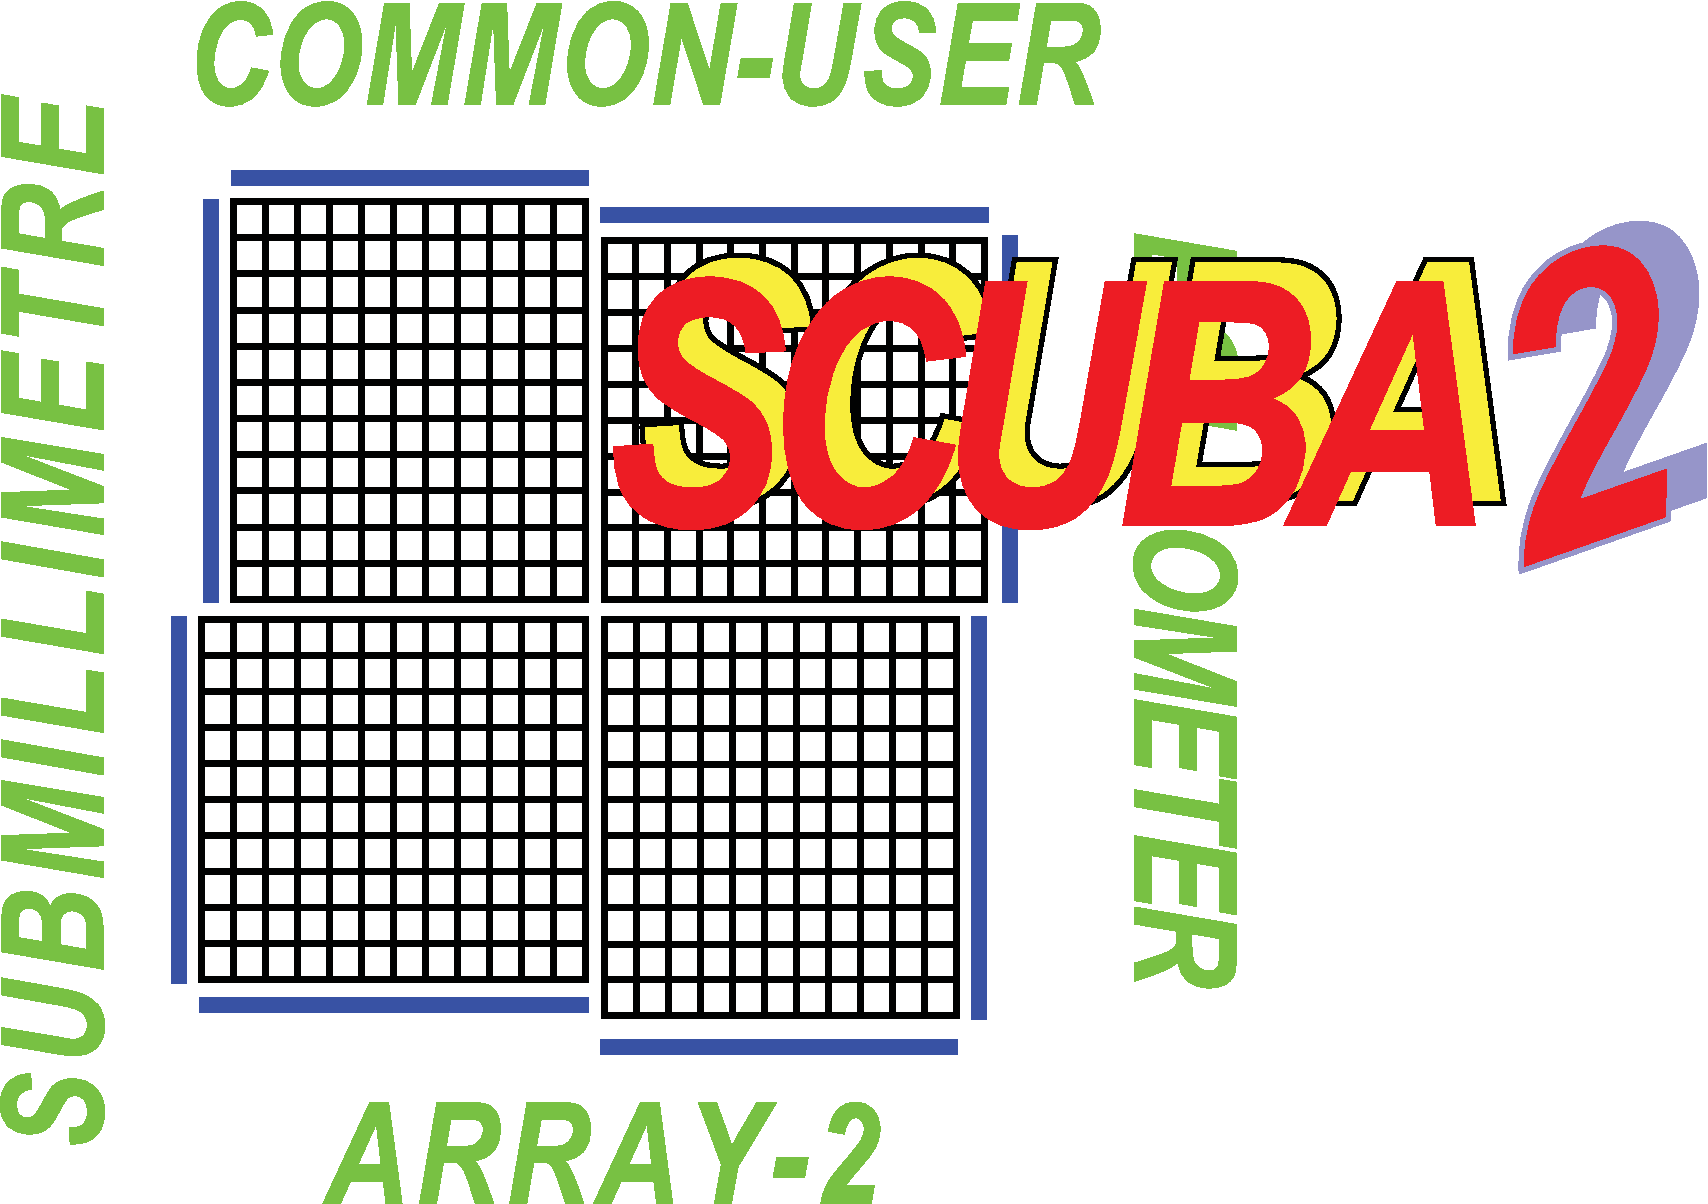
\includegraphics[width=0.7\textwidth]{sc21_s2logo}}
\end{verbatim}

The \texttt{startitlepic}, \texttt{stardocmanual},
\texttt{stardocversion} can always be left out if you have nothing to
fill them in with. The \texttt{stardocabstract} can be left out if you
give the class option \texttt{noabs}.

These commands must be given in the document preamble (i.e.\ before
the \verb+\begin{document}+ command).
% \stardoc stuff

\section{Class specific Macros}

\texttt{aligndesc}


scpushright

noteroutine/classitem/menuitem

\texttt{terminalv}


Already defined abbreviations.

tip boxes

slboxes

sllongtables

\section{hyperlinks}

internal

external (normal)

external to other starlink documents

\section{SST}


\section{Images}
Automatically converted by htlatex script.

Other formats are possible if needed.

Size as a percentage of body width should be same as in latex (as a
percentage of linewidth).

Cannot rotate (i.e. can't use angle= modifier to includegraphics
command)

Generally with floats: don't spend hours carefully tweaking exactly
where it comes out on the latex output. Someone else will come along
and add a couple of new paragraphs near the start, and all your work
will be undone. In html output, the float will occur whereever you
placed it in the text, so ensure that that makes sense. You can use
the usual position modifiers, but note that try not to limit latex too
much in where it can put the float.

If pdflatex really keeps putting the float much later than you want,
then use \verb+\clearpage+ which will flush out all the floats. This
can give you a page with an annoying amount of blank space, but for
technical documentation that is much better than producing a hard to
maintain document.

\section{What to avoid}

nesting maths/pictures -- goes weird.

minipages -- can be used but are finicky.

very unusual latex (TeX4ht's default customisations are a lot better
for more common packages...)

htlatex require more braces around \textunderscore and \^ than
pdflatex insists upon.

indexes currently don't produce any output in html, and if you add an
index to an existing document you'll probably have to edit the build
script before it will produce one.


\section{Issues}

How to use \verb+\part+

If you really need a minipage...

maths issues -- check with and without mathjax?

Can't rotate images -- must do manually before.

\section{Customisations}

generally okay, but check it works in html too.

Don't try and completely change appearance.

File a bug if appearance is broken -- sometimes it'll be an issue you
have to work around, sometimes an easy to fix solution will be found.



\section{Template File}

A template file you can copy if staring a new starlink document can be found at.

\appendix

\section{Source for this document}

\end{document}
